\documentclass[xcolor=pdflatex,dvipsnames,table]{beamer}
\usepackage{epsfig,graphicx}
\usepackage{palatino}
\usepackage{fancybox}
\usepackage{relsize}
\usepackage[procnames]{listings}
\usepackage{hyperref}
\usepackage{qtree} % needed?
\usepackage{booktabs}
\usepackage{dirtree}
\usepackage[normalem]{ulem}


% fatter TT font
\renewcommand*\ttdefault{txtt}
% another TT, suggested by Alex
% \usepackage{inconsolata}
% \usepackage[T1]{fontenc} % needed as well?


\newcommand{\scale}{0.7}

\newcommand{\todo}[1]{{\emph{TODO: #1}}}
\newcommand{\martin}[1]{{\color{blue} Martin: #1}}
\newcommand{\abcdef}[1]{{\color{red} Author2: #1}}

% uncomment following for final submission
%\renewcommand{\todo}[1]{}
%\renewcommand{\martin}[1]{}
%\renewcommand{\author2}[1]{}

\newcommand{\code}[1]{{\texttt{#1}}}

\hypersetup{
  linkcolor  = black,
%  citecolor  = blue,
  urlcolor   = blue,
  colorlinks = true,
}

\beamertemplatenavigationsymbolsempty
\setbeamertemplate{footline}[frame number]





\newif\ifbook
% shared in slides and book

\lstdefinelanguage{chisel}{
  morekeywords={abstract,case,catch,class,def,%
    do,else,extends,false,final,finally,%
    for,if,implicit,import,match,mixin,%
    new,null,object,override,package,%
    private,protected,requires,return,sealed,%
    super,this,throw,trait,true,try,%
    type,val,var,while,with,yield},
  otherkeywords={=>,<-,<\%,<:,>:,\#,@},
  sensitive=true,
  morecomment=[l]{//},
  morecomment=[n]{/*}{*/},
  morestring=[b]",
  morestring=[b]',
  morestring=[b]"""
}

\usepackage{color}
\definecolor{dkgreen}{rgb}{0,0.6,0}
\definecolor{gray}{rgb}{0.5,0.5,0.5}
\definecolor{mauve}{rgb}{0.58,0,0.82}

% Default settings for code listings
\ifbook
\lstset{%frame=lines,
  language=chisel,
  aboveskip=3mm,
  belowskip=3mm,
  showstringspaces=false,
  columns=fixed, % basewidth=\mybasewidth,
  basicstyle={\small\ttfamily},
  numbers=none,
  numberstyle=\footnotesize,
  % identifierstyle=\color{red},
  breaklines=true,
  breakatwhitespace=true,
  procnamekeys={def, val, var, class, trait, object, extends},
  % procnamestyle=\ttfamily,
  tabsize=2,
  float
}
\else
\lstset{%frame=lines,
  language=chisel,
  aboveskip=3mm,
  belowskip=3mm,
  showstringspaces=false,
  columns=fixed, % basewidth=\mybasewidth,
  basicstyle={\small\ttfamily},
  numbers=none,
  numberstyle=\footnotesize\color{gray},
  % identifierstyle=\color{red},
  keywordstyle=\color{blue},
  commentstyle=\color{dkgreen},
  stringstyle=\color{mauve},
  breaklines=true,
  breakatwhitespace=true,
  procnamekeys={def, val, var, class, trait, object, extends},
  procnamestyle=\ttfamily\color{red},
  tabsize=2,
  float
}
\fi

\lstnewenvironment{chisel}[1][]
{\lstset{language=chisel,#1}}
{}

\newcommand{\shortlist}[1]{{\lstinputlisting[nolol]{#1}}}

\newcommand{\longlist}[3]{{\lstinputlisting[float, caption={#2}, label={#3}, frame=tb, captionpos=b]{#1}}}

\newcommand{\verylonglist}[3]{{\lstinputlisting[caption={#2}, label={#3}, frame=tb, captionpos=b]{#1}}}


\title{The Vending Machine}
\author{Martin Schoeberl}
\date{\today}
\institute{Technical University of Denmark\\
Embedded Systems Engineering}

\begin{document}

\begin{frame}
\titlepage
\end{frame}

\begin{frame}[fragile]{Overview}
\begin{itemize}
\item Your final grade
\item Online exam
\item The Vending Machine project
\item
\item How many have finished the display multiplexer?
\end{itemize}
\end{frame}

\begin{frame}[fragile]{Your Final Grade}
\begin{enumerate}
\item You lab work, the vending machine
\begin{itemize}
\item What is working (TA checks)
\item Your report
\item Base function is a 10, extra functions needed for a 12
\end{itemize}
\item Written exam
\begin{itemize}
\item Two hour written exam
\end{itemize}
\end{enumerate}
\end{frame}

\begin{frame}[fragile]{Exam Logistics}
\begin{itemize}
\item Online exam with {\bf all materials and Internet access}
\begin{itemize}
\item I assume you will use those resource for doing a pretty good exam result and not for cheating :-)
\item Allowing Internet access actually reflects how we work today
\end{itemize}
\item You need access to the Internet during the two hours
\item I am available if there are questions on Slack and on Zoom
\item You need to be able to submit drawings:
\begin{itemize}
\item Hand drawings and a webcam or smartphone
\item Use a drawing program on your laptop
\item Upload a .pdf (or .jpg), no drawing program specific file formats
\end{itemize}
\end{itemize}
\end{frame}

\begin{frame}[fragile]{Exam Logistics}
\begin{itemize}
\item Online exam with all materials and Internet access
\item DTU has not (yet) decided on a single system
\begin{itemize}
\item There is also not much help (yet) :-(
\item We have to find out
\end{itemize}
\item Digital Exam or
\item within DTU Inside
\item Look at both
\item Do the poll
\end{itemize}
\end{frame}

\begin{frame}[fragile]{Exam Logistics}
\begin{itemize}
\item This is new to all of us: we will manage
\item We will do at least one (better two) test exams to learn the system
\item We will both learn how this works out
\item I will ask similar questions as the questions that will be in the real exam
\end{itemize}
\end{frame}

\begin{frame}[fragile]{Exam Topics and Questions}
\begin{itemize}
\item The pensum (reading lis) is on the \href{http://www2.imm.dtu.dk/courses/02139/}{web site}
\item Compute maximum frequency and delays of a given circuit
\item Answer multiple choice questions on digital design
\item Given a Chisel description of a circuit, draw it
\item Given a circuit drawing, sketch the Chisel description
\item Basically what we have done in the lab
\item No surprises (at least not too many ;-)
\end{itemize}
\end{frame}


%\begin{frame}[fragile]{yyy}
%\begin{itemize}
%\item Hi Martin, I hope it is alright that I'm writing through this forum. But I am extremely nervous regarding the current situation, especially when we can see that DTU is not doing anything to help the students in ANY way. Why have we still not gotten any information regarding the exams? Whereas most of the other universities have already switched to digital exams? We need to soon start preparing soon and it is not helping when we do not have any idea of how things are going to turn out or what DTU plans on doing. I know that it is an ever-changing situation, but so far the situation has been predicted to worsen so why is DTU waiting to throw a "bomb" on its students regarding the exams. I have had already many sleepless night regarding this and would much rather not go down with stress, therefore could you please give us a better picture of what the future holds for us as students at DTU for this semester? 
%
%\item But a HUGE thank you to you for providing such great forums, such as Zoom and Slack for all of us to stay connected and allowing us to work efficiently, but most of my other professors are just ignoring this situation and going on as if we are not going through a global pandemic right now! 
%\end{itemize}
%\end{frame}
%
%\begin{frame}[fragile]{yyy}
%\begin{itemize}
%%\item Jeg ved at det er meget at sp�rge om, men jeg ville gerne vide, om det er mugligt, at f� et eksempel p� hvordan digi examen kommer til at se ud, nu chisel bliver brugt og ikke VHDL. Kunne vi m�ske f� en opgave, der kunne havt v�ret eksamens opgaven? Alts� en opgave med lige s� mange sp�rgsm�l der minder om den vi kommer til at have til examen?
%%Selv ville jeg f�le mig meget mere forberet til examen, hvis jeg kunne se og gennemf�re en examens opgave, f�r den rigtige examen.
%
%\item I know that's a lot to ask, but I wanted to know if it's possible to get an example of what the digi exam will look like, now chisel is being used and not VHDL. Could we maybe get a task that could have been the exam task? So an assignment with just as many questions reminiscent of the one we will have for the exam?
%Even I would feel much more prepared for the exam if I could see and complete an exam assignment before the real exam.
%\end{itemize}
%\end{frame}



\begin{frame}[fragile]{A Vending Machine from 1952}
\begin{figure}
    \centering
    \href{https://en.wikipedia.org/wiki/File:CandiesVendingMachine1952.jpg}{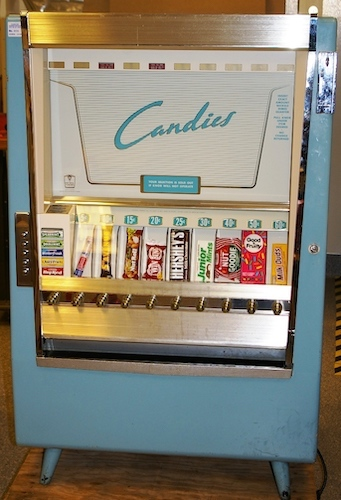
\includegraphics[scale=0.4]{CandiesVendingMachine1952}}

\end{figure}

{\tiny Source: Minnesota Historical Society, \href{https://creativecommons.org/licenses/by-sa/2.0}{CC BY-SA 2.0}}
\end{frame}

\begin{frame}[fragile]{The Vending Machine}
\begin{itemize}
\item Final project is a vending machine
\item Official doument: \href{https://cn.inside.dtu.dk/cnnet/filesharing/download/e712d72e-278e-4fef-a6ed-03eb20134acc}{Vending Machine Specification}
\item Will repeat the overview now
\item Group work
\item Final version shall be run in an FPGA
\item A lot can be done with testing and simulation
\end{itemize}
\end{frame}

\begin{frame}[fragile]{The Vending Machine}
\begin{itemize}
\item Inputs: coins, buy
\item Display: price and current amount
\item Output: release can or error
\item Small challenge to multiplex the display
\item State machine with data path is the \emph{brain} of the VM
\item Guided step by step over several weeks
\end{itemize}
\end{frame}

\begin{frame}[fragile]{Vending Machine Specification I}
\begin{itemize}
\item Sell 1 item and not returning any money
\item Set price with 5 switches (1--31 kr.)
\item Display price on two 7-segment displays (hex.)
\item Accept 2 and 5 kr. (two push buttons)
\item Display sum on two 7-segment displays (hex.)
\begin{itemize}
\item Amount entered so far
\end{itemize}
\item Does not return money, left for the next purchase
\end{itemize}
\end{frame}

\begin{frame}[fragile]{Vending Machine Specification II}
\begin{itemize}
\item Push button \emph{Buy}
\begin{itemize}
\item If not enough money, activate \emph{alarm} as long as buy is pressed
\item If enough money, activate \emph{release item} for as long as \emph{buy}
is pressed and reduce \emph{sum} by the price of the item
\end{itemize}
\item Optional extras (for a 12)
\begin{itemize}
\item Display decimal numbers
\item Supplement alarm by some visuals (e.g., blinking display)
\item Count coins and display an alarm when compartment is full ($>$ 20 coins)
\item Have some text scrolling on the display
\item ...
\item Your ideas :-)
\end{itemize}
\end{itemize}
\end{frame}

\begin{frame}[fragile]{Design and Implementation}
\begin{itemize}
\item Implementation shall be a state machine plus datapath
\item Design your datapath on a sheet of paper
\item Datapath
\begin{itemize}
\item Does add and subtract
\item Contains a register to hold the sum
\item Needs some mulitplexer to operate
\end{itemize}
\item Display needs multiplexing
\begin{itemize}
\item Implemented with some counters and a multiplexer
\end{itemize}
\item Show each part of your design to a TA
\begin{itemize}
\item 7-segment decoder, 7-segment with a counter, display multiplexer, complete vending machine
\end{itemize}
\end{itemize}
\end{frame}

\begin{frame}[fragile]{Draw Figures}
\begin{itemize}
\item Drawings/schematics is another language to describe (digital) circuits
\item Draw, draw, draw boxes and arrows!
\item Use drawing during development
\item If you cannot draw your circuit you do not understand it
\item Use drawings to communicate with the TA
\item Have drawings in your report
\item You will \emph{for sure} need to draw circuits at the exam ;-)
\end{itemize}
\end{frame}



\begin{frame}[fragile]{Vending Machine Design and Implementation Steps}
\begin{itemize}
\item We started in week 5 (now we are at week 10)
\item 2 + 2 + 3 + 3 + 4 + 4 = 18 supervised lab hours
\item 1a. Hexadecimal to 7-segment decoder
\item 1b. 7-segment display with a counter
\item 2. Multiplexed Seven-Segment Display
\item 3. Complete Vending Machine
\item \emph{Show your working design to a TA}
\end{itemize}
\end{frame}

\begin{frame}[fragile]{Final Report}
\begin{itemize}
\item One report per group
\item A single PDF
\begin{itemize}
\item Your group number is part of the file name (e.g., group7.pdf)
\item Code as listing in an appendix (no .zip files)
\item Hand in in DTU Inside
\end{itemize}
\item Content
\begin{itemize}
\item Abstract
\item Preface (Who did what)
\end{itemize}
\begin{enumerate}
\item Introduction and Problem Formulation
\item Analysis and Design
\item Implementation
\item Testing
\item Results
\item Discussion
\item Conclusion
\end{enumerate}
\begin{itemize}
\item List of References
\item Appendix: Chisel code
\end{itemize}
\end{itemize}
\end{frame}

\begin{frame}[fragile]{Material on the Lab GitHub}
\begin{itemize}
\item A top-level component
\item XDC file for Basys pins and frequency
\item A start of a tester generating waveforms
\item A simulation (coming soon)
\item Show it (in IntelliJ)
\end{itemize}
\end{frame}

\begin{frame}[fragile]{Questions on Final Project?}
\end{frame}


\begin{frame}[fragile]{Summary}
\begin{itemize}
\item We are in challenging times
\item Online exam will be challenging
\item We will prepare for it
\item Try to be not afraid of this
\item You will NOT fail because of issues with the online exam
\item Have a good time with your Vending Machine construction
\end{itemize}
\end{frame}



\end{document}

%\begin{frame}[fragile]{xxx}
%\begin{itemize}
%\item yyy
%\end{itemize}
%\end{frame}
